\begin{center}
\begin{longtable}{ |l|l| } 
 \hline
 Attribute & Description\\ 
 \hline
 teamId & ID of the team\\ 
 \hline
 name & name of the team\\ 
 \hline
 teamCreationTime & time when team was created\\ 
 \hline
 teamEndTime & time when last member left the team\\ 
 \hline
 strength & how strong the team is (based on performance)\\ 
 \hline
 currentLevel & current level of the team\\ 
 \hline
\caption{team.csv}
\end{longtable}
\end{center}

Team dataframe has no missing data.
\begin{figure}[H]
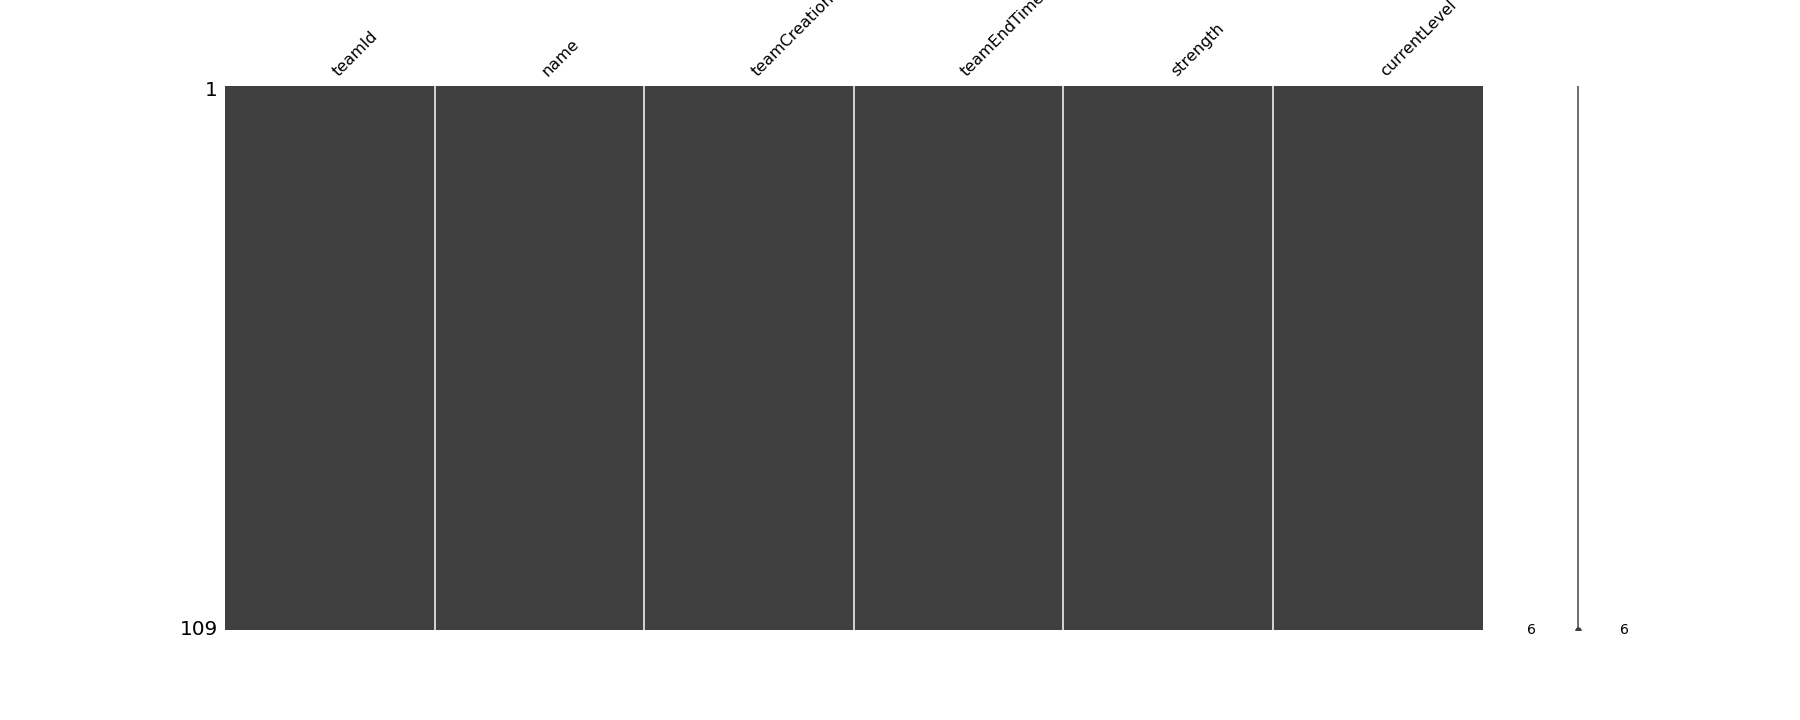
\includegraphics[scale=0.25]{img/Graphs/team/missingno_team.png}
\centering
\caption{missingno\_team}
\label{fig:missingno_team}
\end{figure}


% \begin{figure}[H]
% 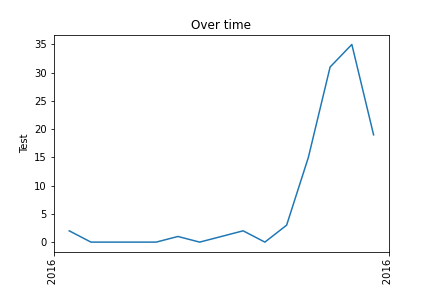
\includegraphics[scale=0.85]{img/Graphs/team/timeseries_team.png}
% \centering
% \caption{timeseries\_team}
% \label{fig:timeseries_team}
% \end{figure}

Analysing team creation time with team end time, we can see something odd. Blue line (representing team creation time) is showcasing how teams were created. Growth was slow, until it expend a lot. By that logic, there should be some teams that were ended (orange line). This can be seen from the start how teams were created and ended, but after a while there seems to be nothing regarding ending of the teams.

With this information, we can conclude two things:
\begin{itemize}
    \item As with time series from above, this one is effected as well,
    \item There seems to be missing data (as we have the data but it is wrong) for team end date since it straight up ends in the middle of the graph.
\end{itemize}
\begin{figure}[H]
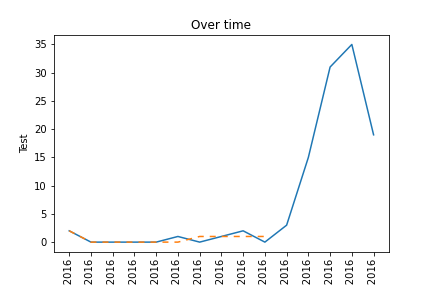
\includegraphics[scale=0.85]{img/Graphs/team/timeseries2_team.png}
\centering
\caption{timeseries2\_team}
\label{fig:timeseries2_team}
\end{figure}

The strongest teams on the graph do not appear on the list of the biggest teams. What is interesting is team with id 9, they are 3rd in terms of strength (Figure \ref{fig:teamStrength_team}) and in terms of spending ( Figure\ref{fig:histogram_buyClicks}). This team appears to spend the most and be the strongest at the same time being 4th biggest team in terms of members (Figure \ref{fig:adClicks_tree_map}).
\begin{figure}[H]
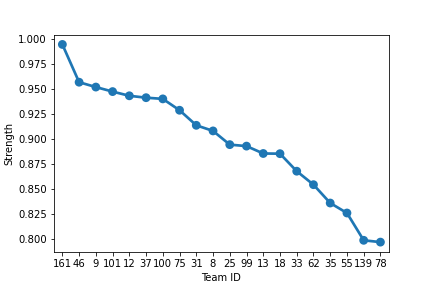
\includegraphics[scale=0.85]{img/Graphs/team/teamStrength_team.png}
\centering
\caption{teamStrength\_team}
\label{fig:teamStrength_team}
\end{figure}

Teams with lower strength do not appear in the biggest team section. But 4th weakest team appears to be on the lower section on spending.
\begin{figure}[H]
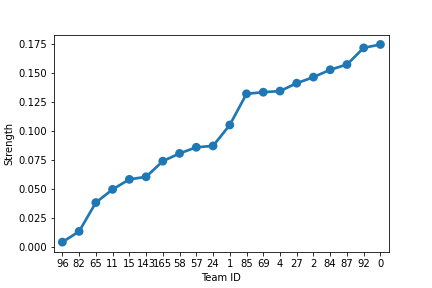
\includegraphics[scale=0.85]{img/Graphs/team/teamStrength2_team.png}
\centering
\caption{teamStrength2\_team}
\label{fig:teamStrength2_team}
\end{figure}